\chapter{基于知识图谱的IT运维辅助系统设计与实现}
实时运行的集群中存在着大量的组件与实时数据,IT运维人员面对海量的信息需要消耗大量精力和时间逐步查询分析多源的繁杂数据。一个基于知识图谱的IT运维辅助系统可以有效地辅助运维人员,帮助其及时发现集群异常并预测可能出现的故障,从而大大降低了运维难度。

本章基于第三章、第四章和第五章提出的各个方法模型,设计并实现了一个基于知识图谱的IT运维辅助系统,并对设计与实现过程展开了细致地描述。本章共分4小节来介绍系统,介绍的内容包括需求分析、系统总体设计、系统详细实现和系统测试。
% 本文设计实现的系统通过jaeger\cite{mengistu2020distributed}、prometheus\cite{padgham2002prometheus}、阿里云公开API等方式获取集群拓扑结构、微服务间拓扑结构、日志数据和指标时序数据,将集群实时运行状态可视化。随后,历史监测数据被按故障类型分组,经过事件因果关系挖掘模型构建了每种故障对应的组件-事件知识图谱。基于构建的组件-事件知识图谱,利用上文提出的表示学习模型和故障预测模型,本系统可以根据实时发生的事件序列预测可能会发生的故障,提醒运维人员及时采取应对措施。


\section{需求分析}\label{need-analysis}
本节详细介绍基于知识图谱的IT运维辅助系统需要满足的需求,包括功能性需求和非功能性需求。功能性需求是指IT运维辅助系统要实现的功能,而非功能性需求是指该系统应当满足的除功能性需求之外的其他需求。
\subsection{功能性需求}
本系统主要目的是辅助IT运维人员,降低实际运维的难度。因此,在系统实现前,本文咨询了IT运维人员,进行了详细的需求调研,总结了IT运维辅助系统的三大功能需求:实时集群状态查询、组件-事件知识图谱查询及调优、实时故障预测。图\ref{user-need}为本章IT运维辅助系统用例图。
\begin{figure}[htbp]
    \centering
    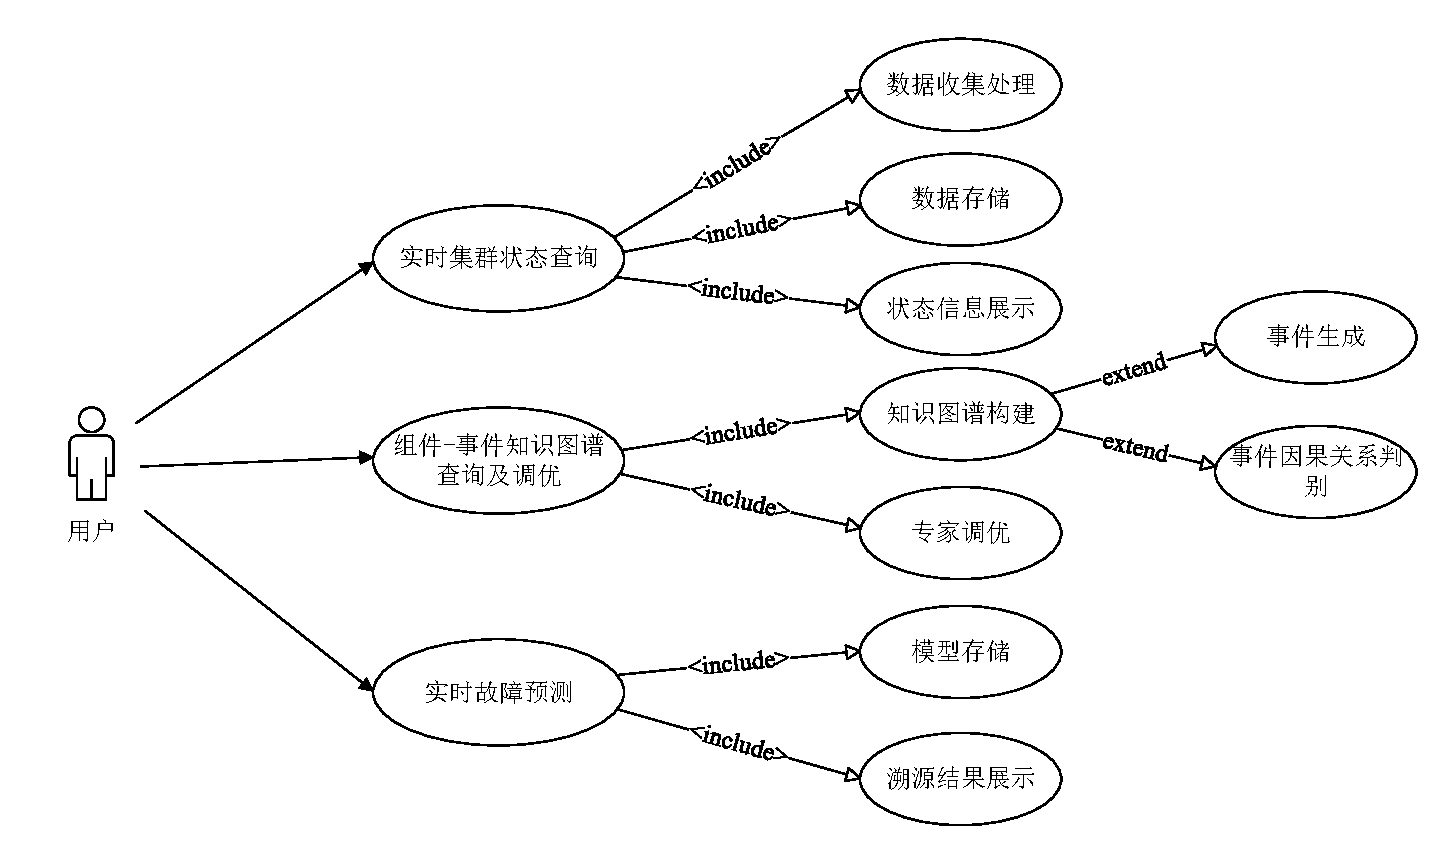
\includegraphics[width=0.98\textwidth]{user-need.pdf}
    \caption{IT运维辅助系统用例图\label{user-need}}
\end{figure}

(1)实时集群状态查询

分布式集群往往包含着上千个组件,每个组件有其特异的属性信息。另外,每个组件会实时产生不同种类的信息:硬件组件会产生内存、读写、CPU 等时序数据,软件组件会产生文本类的日志数据。在分布式集群实际运转时,每秒钟会产生万级的多源异构数据。

IT运维人员在实际工作中,需要调用不同接口,使用不同的开源软件才能全方面的了解每个组件的状态。繁琐的集群状态查询过程,不仅消耗了IT运维人员大量的精力,还会导致运维人员错失最佳的故障解决时机。因此,IT运维人员需要一个能够全面便捷地获取系统状态信息的查询系统。这个集群状态查询系统需要整合多个接口,收集各种状态数据,并将这些数据存储起来。另外,该系统需要提供简洁的查询界面,方便IT运维人员直观地操作。

(2)组件-事件知识图谱查询及调优

组件-事件知识图谱直观地展示了故障触发过程,包含着丰富的运维知识。运维人员在实际工作时,需要查询这些知识图谱,获取运维知识,指导下一步运维工作。系统需要根据第三章的组件-事件知识图谱构建流程,在后台从历史数据沉淀出组件-事件知识图谱。在知识图谱构建时,需要将多源异构数据转为统一规范的事件类型数据,并调用分类器获取事件间因果关系。这种依靠机器学习构建组件-事件知识图谱的方式,虽然能够快速沉淀出可用的故障触发知识,但始终不能做到完全精准,需要运维人员介入,进行少量的人工调优。基于以上分析,本系统需要构建并展示组件-事件知识图谱,方便IT运维人员查询,也方便其对知识图谱进行验证与调优。

(3)实时故障预测

在实际运维工作中,运维人员很难预知是否会有故障发生,往往是在故障发生后采取修复工作。这样解决已发生故障的工作模式,很难避免故障带来的损失。因此,本系统需要提供实时故障预测的功能,能够结合组件-事件知识图谱和实时的运行状态数据,给出准确具体的故障预测结果。为了实现实时故障预测,本系统需要存储多个模型,并给出故障预测结果的可视化展示。


\subsection{非功能性需求}
IT运维辅助系统除了需要满足上节所提的功能,还要满足以下非功能需求:

% (1)故障预测结果要具体准确,系统除了要预测是否会出现故障,还要给出具体会出现的故障,并且预测结果准确率要高。
(1)各个查询接口返回结果要迅速,需要在2s内给出查询结果。

(2)故障预测过程要迅速,系统需要根据实时产生的数据,在5s的响应时间内给出预测结果。


\section{系统总体设计}
本节进行了系统的总体设计,首先给出了系统的总体框架图,随后介绍了各个功能模块的设计。
\subsection{系统总体框架图}
本系统使用B/S(Browser/Server)架构,即用户使用浏览器请求服务,后台服务器响应返回结果的工作模式。B/S整体架构分为三个层次,包括模型、视图和控制器。其中,模型负责实现业务功能逻辑,即按照功能需求整合转换数据形式;视图则将数据可视化,即把模型返回的数据直观地易于理解地展示出来;控制器则是从视图中接收用户输入的数据,并将数据传送给模型。另外,按照系统功能又可以把系统结构划分为数据层、业务逻辑层和交互层。图\ref{system-constructure}展示了这三层结构。
% \begin{itemize}
%     \item [(1)]数据层。本系统的数据层主要用于存储各种数据,使用了三种存储数据库,用于存储不同类型的数据。Kafka用于缓存大量的微服务实时访问请求,这部分数据会被用于生成微服务间拓扑关系;Neo4j用于存储生成的组件-事件知识图谱;阿里云SLS用于存储日志数据和指标时序数据。
%     % 包含了日志数据、指标时序数据、集群组件拓扑和微服务间拓扑。这四类数据有不同的获取方式,具体获取方式在小节\ref{data-collect-way}进行了具体描述。
%     \item [(2)]业务逻辑层。业务逻辑层连接了数据层与交互层,包含了算法模型和业务逻辑。该层由多个模块协同工作实现系统功能,分为状态监测模块、组件-事件知识图谱构建模块和故障预测模块。每个模块的具体功能在下面几小节展开介绍。
%     \item [(3)]交互层。交互层将业务逻辑层数据可视化地直观展示在前端页面,并支持用户操作数据。本系统交互层主要分为三部分:组件-事件知识图谱查询及调优页面、实时集群状态查询页面和故障预测页面。
% \end{itemize}

(1)数据层。本系统的数据层主要用于存储各种数据,使用了三种存储数据库,用于存储不同类型的数据。Kafka用于缓存大量的微服务实时访问请求,这部分数据会被用于生成微服务间拓扑关系;Neo4j用于存储生成的组件-事件知识图谱;阿里云SLS用于存储日志数据和指标时序数据。

    % 包含了日志数据、指标时序数据、集群组件拓扑和微服务间拓扑。这四类数据有不同的获取方式,具体获取方式在小节\ref{data-collect-way}进行了具体描述。
(2)业务逻辑层。业务逻辑层连接了数据层与交互层,包含了算法模型和业务逻辑。该层由多个模块协同工作实现系统功能,分为状态监测模块、组件-事件知识图谱构建模块和故障预测模块。每个模块的具体功能在下面几小节展开介绍。

(3)交互层。交互层将业务逻辑层数据可视化地直观展示在前端页面,并支持用户操作数据。本系统交互层主要分为三部分:组件-事件知识图谱查询及调优页面、实时集群状态查询页面和故障预测页面。

\begin{figure}[htbp]
    \centering
    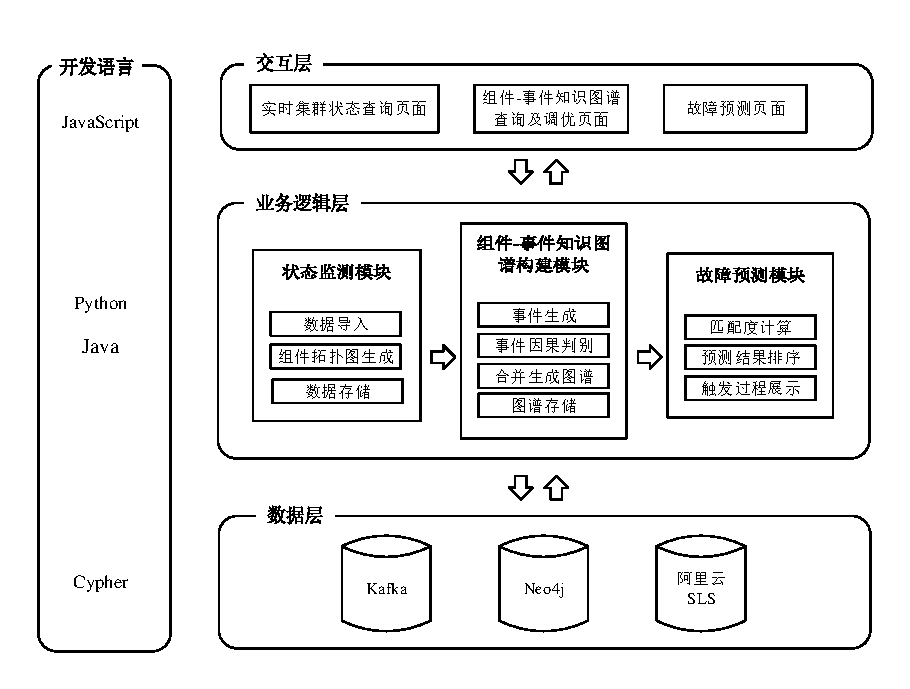
\includegraphics[width=0.8\textwidth]{system-constructure.pdf}
    \caption{IT运维辅助系统框架图\label{system-constructure}}
\end{figure}
% \begin{figure}[htbp]
%     \centering
%     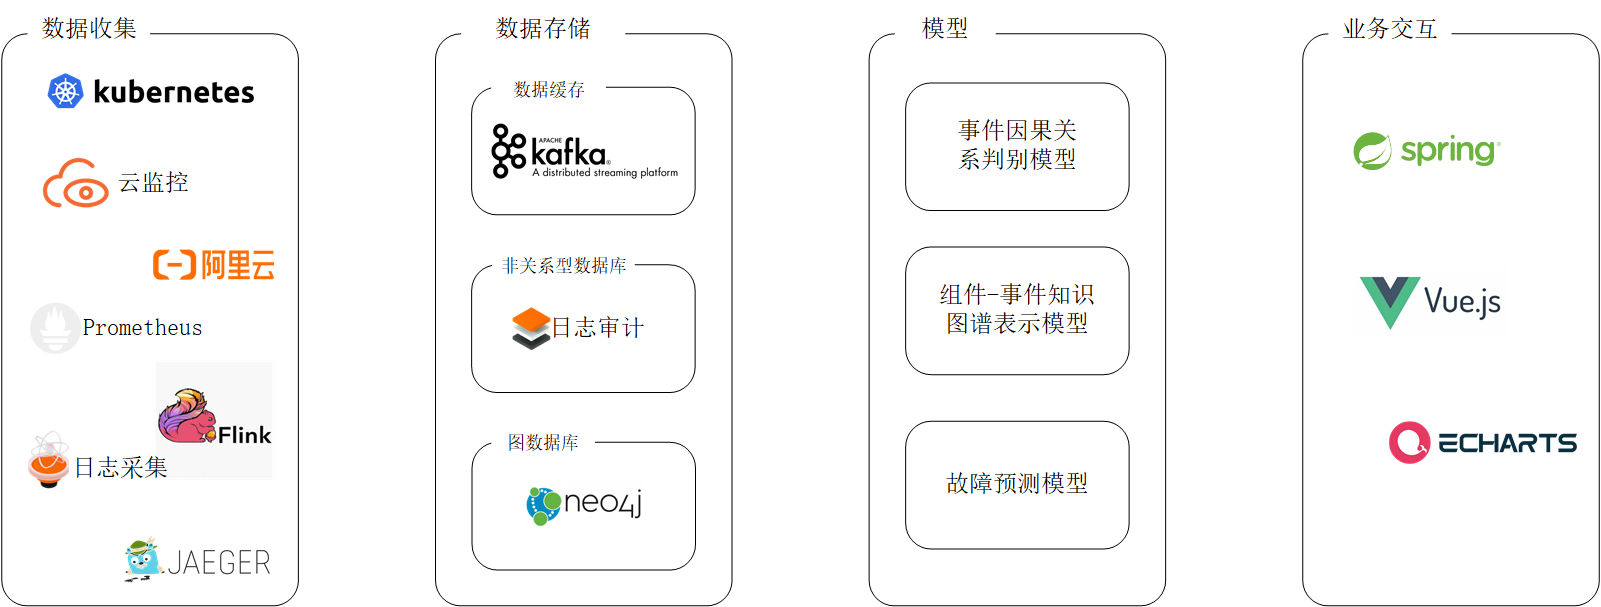
\includegraphics[width=0.8\textwidth]{system-technology.png}
%     \caption{IT运维辅助系统相关工具\label{system-technology}}
% \end{figure}

% \subsection{功能模块设计}\label{system-function}
\subsection{状态监测模块概要设计}
本模块主要负责将不同来源、不同种类的数据整合起来,减少IT运维人员查询数据的难度。该模块需要设计并实现数据导入、组件拓扑图生成和数据存储三部分,分别如下:
% \begin{itemize}
%     \item [(1)]数据导入部分要使用不同的API,不同的中间件,获取不同种类的数据,包括日志数据、指标时序数据、组件属性数据、微服务请求数据;
%     \item [(2)]组件拓扑图生成部分需要分析组件属性、微服务请求数据,生成组件间拓扑图;
%     \item [(3)]数据存储部分负责数据持久化,需要整理不同形式的数据,并根据数据特性存入不同的数据库中。
% \end{itemize}

(1)数据导入部分要使用不同的API,不同的中间件,获取不同种类的数据,包括日志数据、指标时序数据、组件属性数据、微服务请求数据;

(2)组件拓扑图生成部分需要分析组件属性、微服务请求数据,生成组件间拓扑图;

(3)数据存储部分负责数据持久化,需要整理不同形式的数据,并根据数据特性存入不同的数据库中。

\subsection{组件-事件知识图谱构建模块概要设计}
本模块的主要功能是从历史数据中沉淀生成组件-事件知识图谱。本模块需要设计并实现4个子功能:
% \begin{itemize}
%     \item [(1)]首先,该模块需要整理日志数据、指标时序数据,转化为统一格式的事件类型数据;
%     \item [(2)]随后,该模块需要调用机器学习模型,判别事件间是否有因果关系;
%     \item [(3)]然后,该模块需要合并生成的事件因果关系,生成抽象事件层图谱,再结合组件拓扑图得到组件-事件知识图谱;
%     \item [(4)]最后,该模块要把生成的组件-事件知识图谱存入Neo4j中,以保证可以被其他模块调用。
% \end{itemize}

(1)首先,该模块需要整理日志数据、指标时序数据,转化为统一格式的事件类型数据;

(2)随后,该模块需要调用机器学习模型,判别事件间是否有因果关系;

(3)然后,该模块需要合并生成的事件因果关系,生成抽象事件层图谱,再结合组件拓扑图得到组件-事件知识图谱;

(4)最后,该模块要把生成的组件-事件知识图谱存入Neo4j中,以保证可以被其他模块调用。

\subsection{故障预测模块概要设计}
本模块的主要功能是实时预测集群是否会发生故障,并给出故障预测结果排名。本模块需要设计并实现3个部分,分别为匹配度计算,预测结果排序和触发过程展示,具体如下:
% \begin{itemize}
%     \item [(1)]在匹配度计算部分,每个故障类型的组件-事件知识图谱,会分别与实时事件序列进行匹配度计算,匹配度越高意味着越有可能发生对应类型的故障。
%     \item [(2)]在预测结果排序部分,本模块会根据匹配度降序排列候选故障类型,当所有匹配度均小于阈值时,会认为不会有故障发生。
%     \item [(3)]在触发过程展示部分,本模块会结合组件-事件知识图谱和实时事件序列,给出可能会发生的故障的触发过程。
% \end{itemize}

(1)在匹配度计算部分,每个故障类型的组件-事件知识图谱,会分别与实时事件序列进行匹配度计算,匹配度越高意味着越有可能发生对应类型的故障。

(2)在预测结果排序部分,本模块会根据匹配度降序排列候选故障类型,当所有匹配度均小于阈值时,会认为不会有故障发生。

(3)在触发过程展示部分,本模块会结合组件-事件知识图谱和实时事件序列,给出可能会发生的故障的触发过程。

% 系统各功能模块已在图\ref{system-constructure}中业务逻辑层展示,分为:a.事件生成模块、b.组件拓扑生成模块、c.集群状态监测模块、d.事件因果判别模块、e.组件-事件知识图谱生成模块、f.故障预测模块。下面具体介绍这些模块的功能:
% \begin{itemize}
%     \item [a.]事件生成模块:收集各种实时的系统运行数据,将数据转化为统一规范的事件类型数据。
%     \item [b.]组件拓扑生成模块:分析集群组件属性信息列表,根据其中表明了集群组件关系的字段,生成集群组件拓扑。而微服务间的拓扑则利用其实际工作时的访问关系生成。
%     \item [c.]集群状态监测模块:根据事件发生所在的组件位置,将前两个模块数据关联起来,得到可视化的集群运行状态图。
%     \item [d.]事件因果关系判别模块:借助事件因果关系判别模型,分析事件间是否具有因果关系。
%     \item [e.]组件-事件知识图谱生成模块:从某类故障的历史数据中沉淀出包含组件依赖关系、组件事件产生关系和抽象事件因果关系的组件-事件知识图谱。
%     \item [f.]故障预测模块:基于集群状态监测模块所收集的事件序列,联合组件-事件知识图谱,预测未来可能发生的故障。
% \end{itemize}
\section{系统详细实现}
本节介绍系统的详细实现过程,分为3小节展开介绍,分别为状态监测模块详细实现、组件-事件知识图谱构建模块详细实现和故障预测模块详细实现。

\subsection{状态监测模块详细实现}\label{data-collect-way}
状态监测模块从多个源头获取多种类别的数据。本模块通过处理收集到的数据,生成共计4类数据,包括集群拓扑结构、微服务拓扑结构、日志数据、指标时序数据。下面分为4部分分别介绍这四种数据的实际收集、处理、存储流程。
% \subsubsection{集群拓扑结构}

第一部分为集群拓扑结构数据,分为以下步骤:
\begin{itemize}
    \item [(1)]系统开发时,引入阿里云提供的SDK核心库和组件的Maven项目依赖。
    \item [(2)]编写多线程代码调用不同组件的数据请求方法并设置参数,再保存方法返回的Json数据。如调用方法$DescribeImagesRequest(.)$,设置要查询的镜像类型$setImageOwnerAlias(.)$,就会返回对应镜像的Json格式的基本信息。
    \item [(3)]分析返回的Json数据,读取指定字段值。返回的Json数据不同字段包含着不同类型的信息,如字段$ ImageId: freebsd\_11\_02\_64\_30G\_alibase\_20190722.vhd$表明了镜像的唯一标识符;$OSNameEn: FreeBSD  11.2 64 bit$表明了系统名称;$VpcId:vpc—2zeuphj08tt7q3brd****$表明了ECS所在VPC。
    \item [(4)]按获取的字段信息构建实体属性列表,和组件间关联拓扑。
\end{itemize}

% (1)系统开发时,引入阿里云提供的SDK核心库和组件的Maven项目依赖。

% (2)编写多线程代码调用不同组件的数据请求方法并设置参数,再保存方法返回的Json数据。如调用方法$DescribeImagesRequest(.)$,设置要查询的镜像类型$setImageOwnerAlias(.)$,就会返回对应镜像的Json格式的基本信息。

% (3)分析返回的Json数据,读取指定字段值。返回的Json数据不同字段包含着不同类型的信息,如字段$ ImageId: freebsd\_11\_02\_64\_30G\_alibase\_20190722.vhd$表明了镜像的唯一标识符;$OSNameEn: FreeBSD  11.2 64 bit$表明了系统名称;$VpcId:vpc—2zeuphj08tt7q3brd****$表明了ECS所在VPC。

% (4)按获取的字段信息构建实体属性列表,和组件间关联拓扑。

% \subsubsection{微服务拓扑结构}
第二部分为微服务拓扑结构的获取。微服务依赖关系虽然在分布式应用的代码逻辑中已清晰规定,但应用的代码属于机密信息且阅读代码时耗过大。为了无需了解应用代码逻辑就可以获取微服务间访问拓扑关系,本系统选用开源Jaeger实时监控微服务间的访问信息,并存储到Kafka中。Jaeger获取微服务拓扑结构流程如图\ref{tracing-generate}所示,其中span的颜色代表了它对应何种微服务。一个Span对应一条微服务被调用的记录,其记录了微服务被标识符为parentSpan中的微服务调用了一次。一个Trace对应着微服务间的一条请求链路。具体步骤如下:
% \begin{figure}[htbp]
%     \centering
%     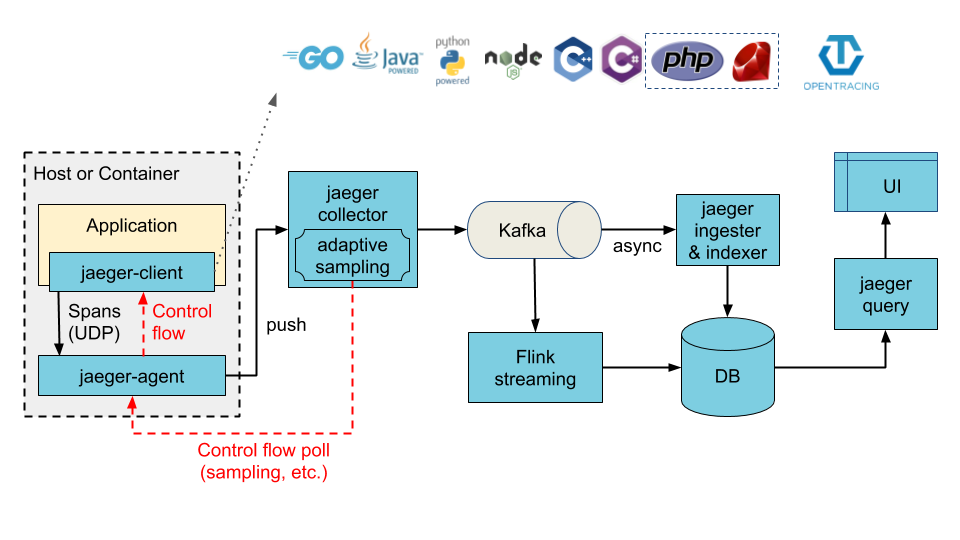
\includegraphics[width=0.8\textwidth]{jaeger-system-constructure.png}
%     \caption{Jaeger架构图\label{jaeger-system-constructure}}
% \end{figure}

% Jaeger架构图如图\ref{jaeger-system-constructure}所示,主要包含以下几个部分:
% \begin{itemize}
%     \item [(1)] \textbf{jaeger client libraries}:jaeger客户端是基于OpenTracing API的特定语言实现的,可通过与OpenTracing集成的各种现有开源框架来检测应用程序,实现分布式跟踪。它会以较小的开销始终在后台开启,不断采样Span并异步传输到Jaeger Agents。采样策略默认为随机采样0.1\%。
%     \item [(2)]\textbf{jaeger agents}:Agent是网络守护程序,负责侦听通过UDP传输的Span,并分批次将Span发送给Collector。另外,它作为一种基础结构组件会被部署到所有主机。
%     \item [(3)]\textbf{Collector}:Collector在接收到Agent传来的Span后,会验证跟踪并为这些Span建立索引,并最终存储起来。Jaeger使用的存储设备是可插拔的,目前支持Cassandra、Elasticsearch和Kafka。
%     \item [(4)]\textbf{Query}:Query是一项从存储中检索微服务依赖信息,并用UI显示的服务。
%     \item [(5)]\textbf{Ingester}:Ingester是负责提供从Kafka读取数据并写入其他存储后端的服务。
% \end{itemize}

\begin{figure}[htbp]
    \centering
    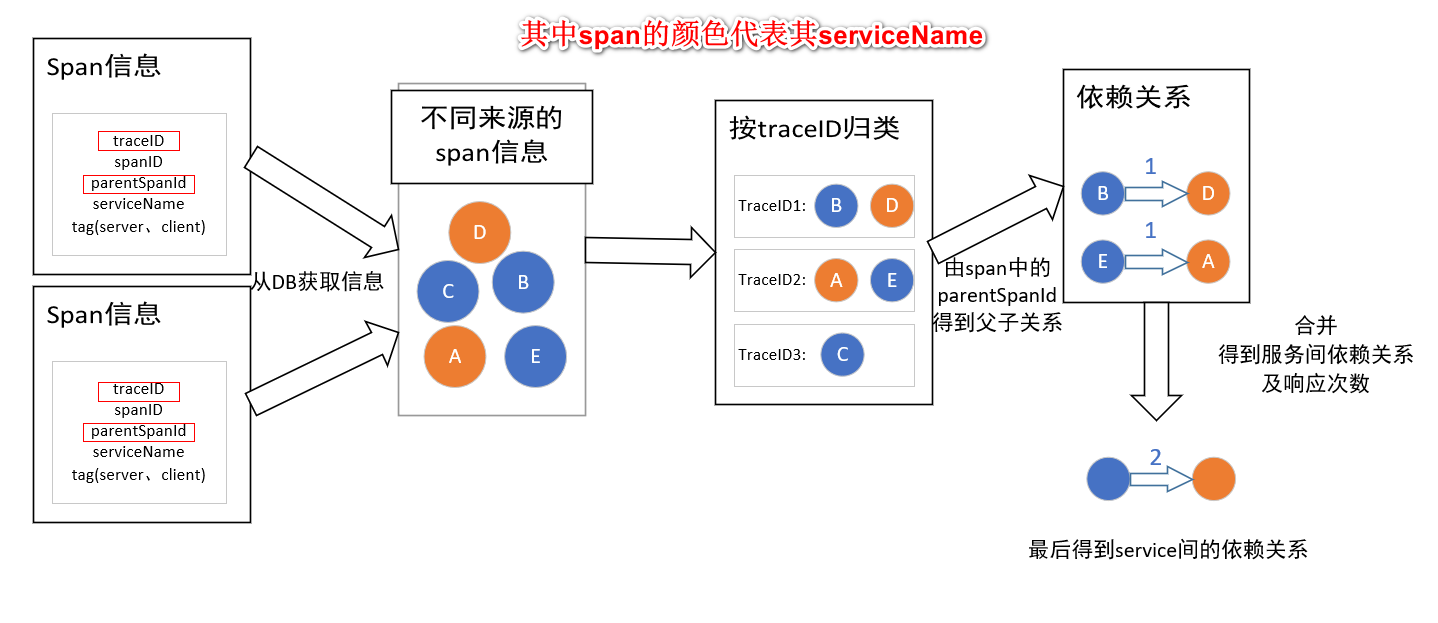
\includegraphics[width=0.8\textwidth]{tracing-generate.png}
    \caption{微服务间依赖图生成流程\label{tracing-generate}}
\end{figure}

\begin{itemize}
    \item [(1)]获取Span数据:从Kafka中读取一个时间段内所有来源的Span。
    \item [(2)]分组Span数据:将所有Span按照traceID分组,这样就获得了traceID到Span集合的映射关系。
    \item [(3)]分析同组Span间依赖关系:遍历每个Span对应的ParentSpanID,得到Span之间的父子依赖关系。
    \item [(4)]生成微服务间依赖关系:根据Span中serviceName信息,将Span间依赖关系映射为微服务间依赖关系。
    \item [(5)]微服务间拓扑图生成:将不同Trace中微服务间依赖关系整合规约,生成微服务拓扑图结构。
\end{itemize}

% (1)获取Span数据:从Kafka中读取一个时间段内所有来源的Span。

% (2)分组Span数据:将所有Span按照traceID分组,这样就获得了traceID到Span集合的映射关系。

% (3)分析同组Span间依赖关系:遍历每个Span对应的ParentSpanID,得到Span之间的父子依赖关系。

% (4)生成微服务间依赖关系:根据Span中serviceName信息,将Span间依赖关系映射为微服务间依赖关系。

% (5)微服务间拓扑图生成:将不同Trace中微服务间依赖关系整合规约,生成微服务拓扑图结构。

% \subsubsection{日志数据}
第三部分为日志数据的收集。日志数据的收集分为以下步骤:
\begin{itemize}
    \item [(1)]日志数据采集。阿里云日志服务(Log Service, SLS)提供了数据投递、查询、消费和采集等功能,可以高效的处理海量日志。在阿里云日志服务中创建Logstore,选择DockerIO、k8s日志等作为数据源,日志服务就会实时将数据汇总收集起来。
    \begin{figure}[htbp]
        \centering
        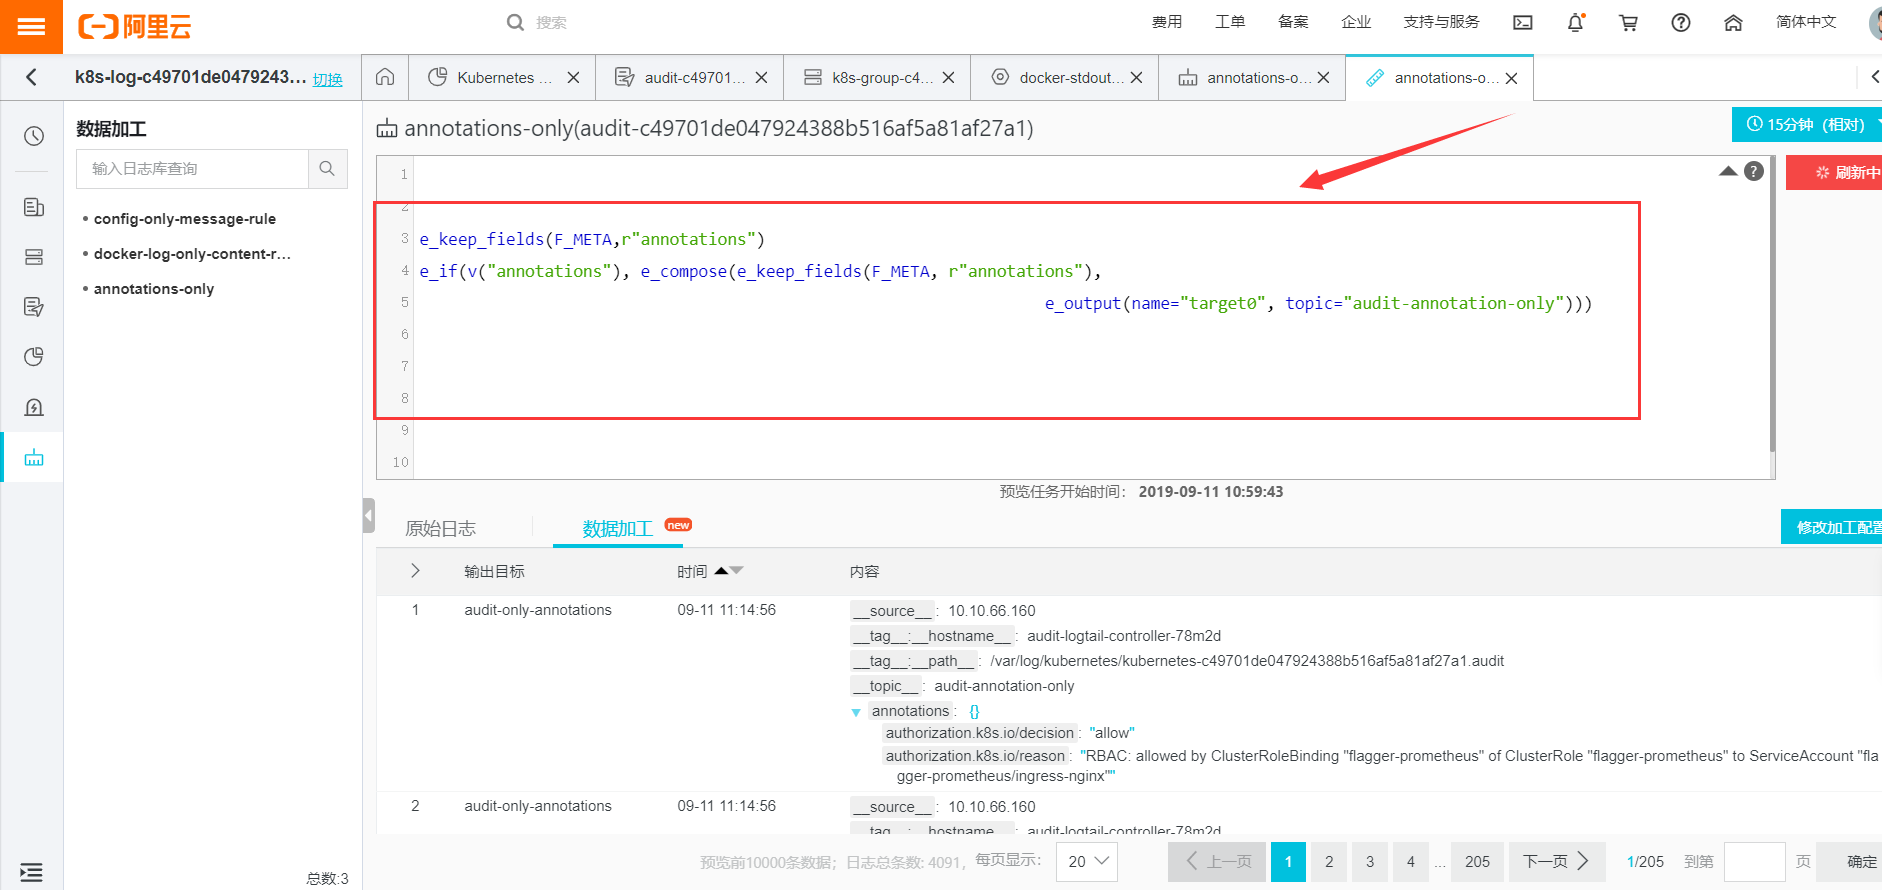
\includegraphics[width=0.7\textwidth]{data-process.png}
        \caption{数据加工指令\label{data-process}}
    \end{figure}
    \item [(2)]日志数据加工。由于原始日志数据包含了很多无效信息,上一步得到的原始日志需要进一步加工处理只保留有效字段信息。加工过程直接使用日志服务的数据加工功能,编写加工命令选取保留的字段,并传输到新的Logstore中即可。如图\ref{data-process}所示图,该数据加工指令只保留了audit数据中的annotation字段。
    % \begin{figure}[htbp]
    %     \centering
    %     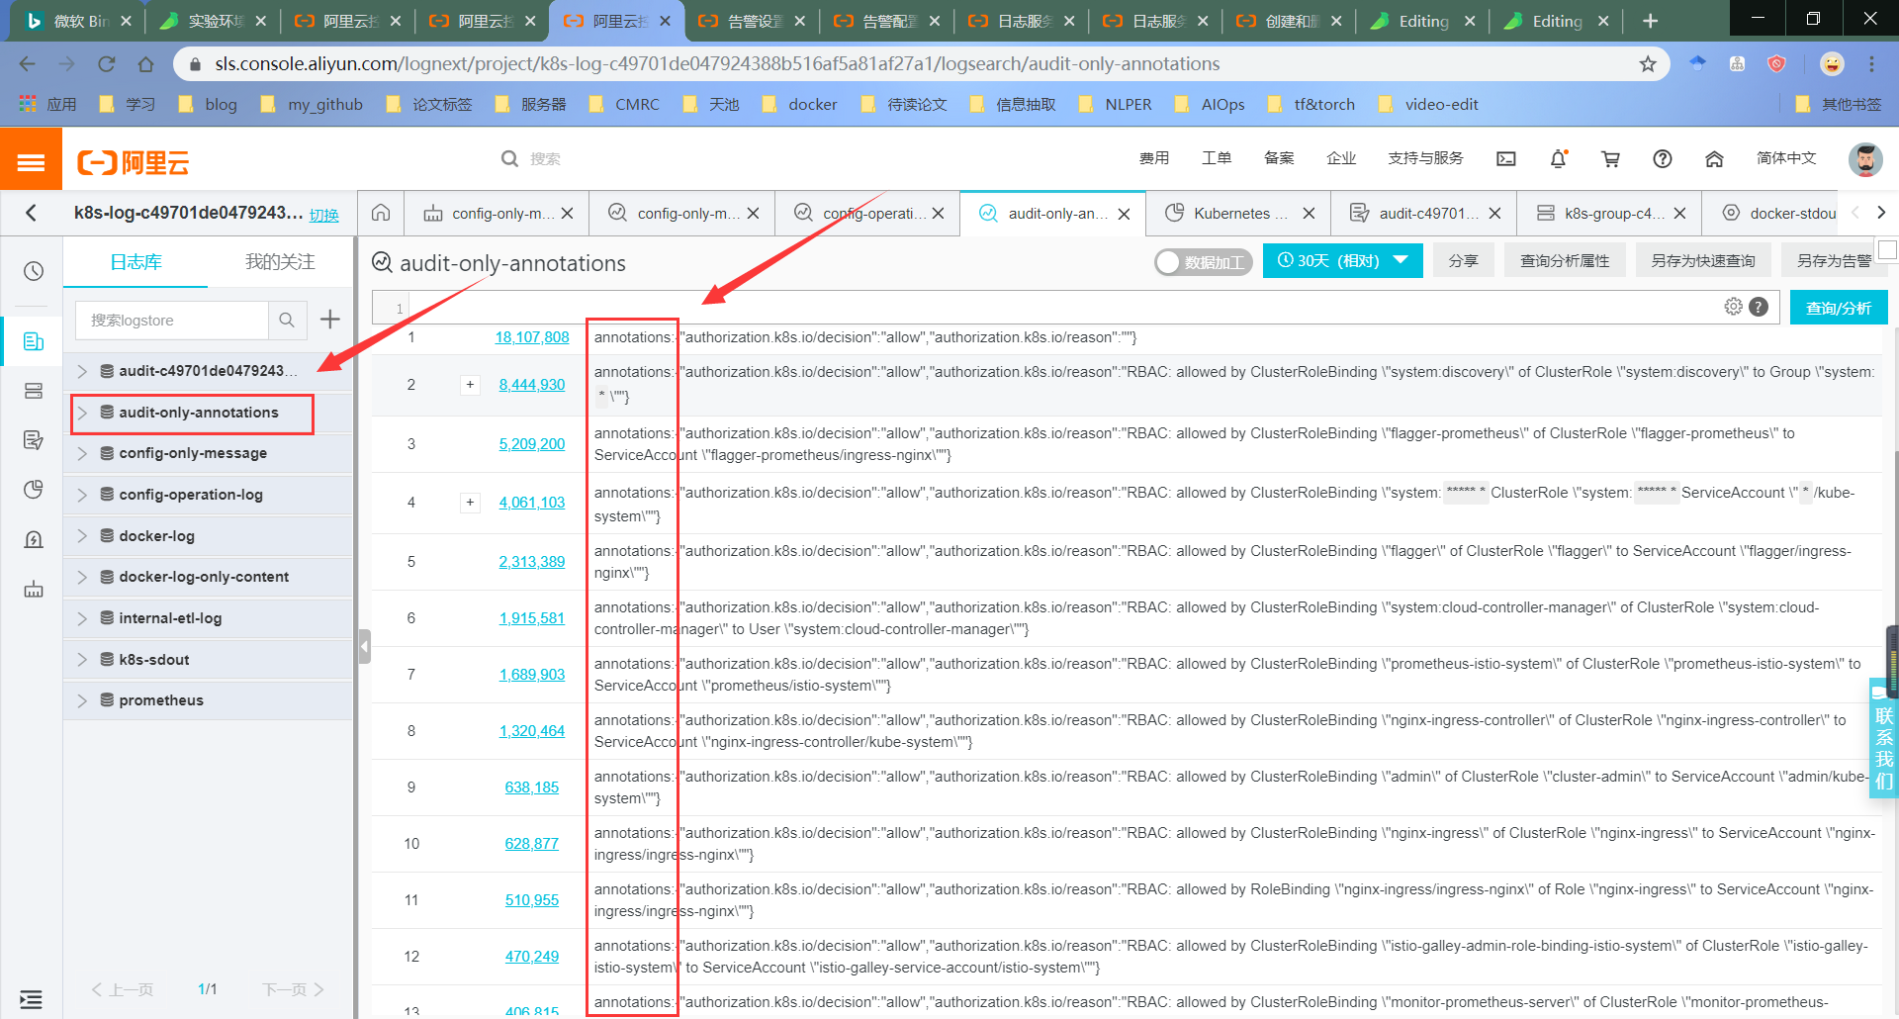
\includegraphics[width=0.7\textwidth]{sls-audit-cluster.png}
    %     \caption{数据加工结果实例\label{sls-audit-cluster}}
    % \end{figure}
    \item [(3)]使用公开API请求日志数据。经过上述步骤,日志数据被存储在日志服务各个Logstore中。当系统需要获取某段时间日志数据时,系统直接使用公开API并设置参数请求即可。如使用函数$PullLogsRequest(project, logStore, shardId, logNum, cursor)$并设置所要消费的project、LogStore和每次读取日志数量logNum等参数,就会返回符合参数约束的日志数据。
\end{itemize}

% (1)日志数据采集。阿里云日志服务(Log Service, SLS)提供了数据投递、查询、消费和采集等功能,可以高效的处理海量日志。在阿里云日志服务中创建Logstore,选择DockerIO、k8s日志等作为数据源,日志服务就会实时将数据汇总收集起来。
%     \begin{figure}[htbp]
%         \centering
%         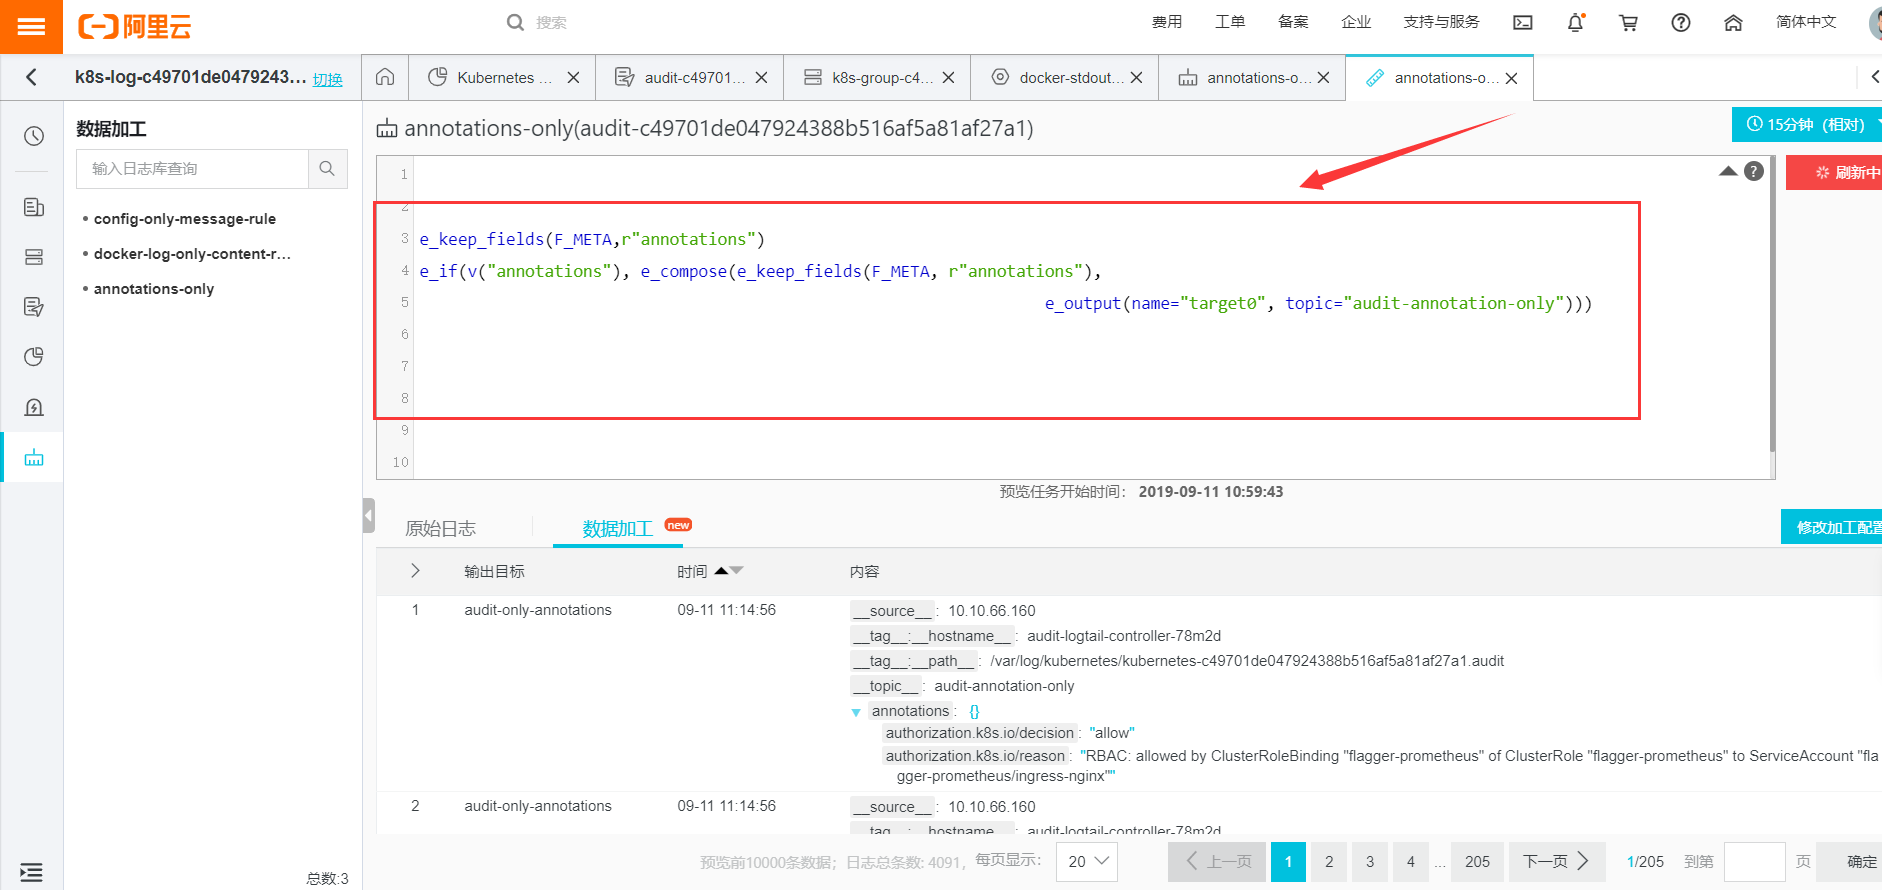
\includegraphics[width=0.7\textwidth]{data-process.png}
%         \caption{数据加工指令\label{data-process}}
%     \end{figure}

% (2)日志数据加工。由于原始日志数据包含了很多无效信息,上一步得到的原始日志需要进一步加工处理只保留有效字段信息。加工过程直接使用日志服务的数据加工功能,编写加工命令选取保留的字段,并传输到新的Logstore中即可。如图\ref{data-process}所示图,该数据加工指令只保留了audit数据中的annotation字段。

% (3)使用公开API请求日志数据。经过上述步骤,日志数据被存储在日志服务各个Logstore中。当系统需要获取某段时间日志数据时,系统直接使用公开API并设置参数请求即可。如使用函数$PullLogsRequest(project, logStore, shardId, logNum, cursor)$并设置所要消费的project、LogStore和每次读取日志数量logNum等参数,就会返回符合参数约束的日志数据。

% \subsubsection{指标时序数据}
第四部分为获取指标时序数据。指标时序数据均为曲线类的数据,在存储形式上,均为一组时间戳到值的映射关系集合。其获取过程如下:
\begin{itemize}
    \item [(1)]指标时序数据监测。在分布式集群中,多种组件都会有指标时序数据,且每个组件上会有不同种类的指标时序数据,如CPU、内存、磁盘吞吐率等。系统选用了Prometheus进行实时的监测。
    \item [(2)]指标时序数据长期存储。由于Prometheus监测得到的指标时序数据不能长期存储(一般只保留14天),系统为了长期存储选择将数据导入日志服务。
    % 图\ref{metric-prometheus}展示了指标时序数据导入日志服务后的结果,可见每条数据都对应着一个时间戳到值的映射关系。
    % \begin{figure}[htbp]
    %     \centering
    %     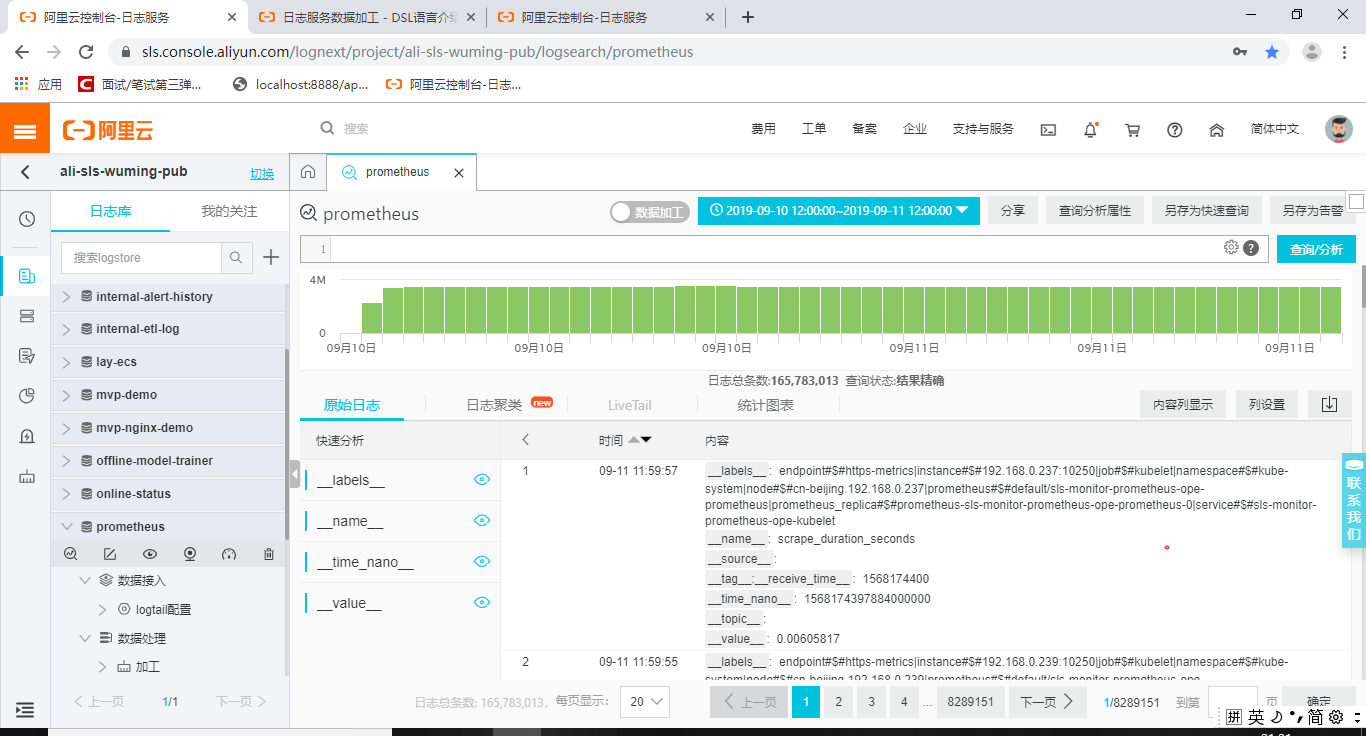
\includegraphics[width=0.8\textwidth]{metric-prometheus.png}
    %     \caption{指标时序数据导入日志服务示例\label{metric-prometheus}}
    % \end{figure}
    \item [(3)]公开API获取指标时序数据。将数据长期存储入日志服务平台后,系统可采用请求日志的API来请求获取指标时序数据。
\end{itemize}

% (1)指标时序数据监测。在分布式集群中,多种组件都会有指标时序数据,且每个组件上会有不同种类的指标时序数据,如CPU、内存、磁盘吞吐率等。系统选用了Prometheus进行实时的监测。

% (2)指标时序数据长期存储。由于Prometheus监测得到的指标时序数据不能长期存储(一般只保留14天),系统为了长期存储选择将数据导入日志服务。

% (3)公开API获取指标时序数据。将数据长期存储入日志服务平台后,系统可采用请求日志的API来请求获取指标时序数据。

\subsection{组件-事件知识图谱构建模块详细实现}
本节介绍实际中构建组件-事件知识图谱的程序流程,如图\ref{graph-constructure-process}所示。用于构建知识图谱的历史故障数据,都已经按照故障类型进行了分组。本模块分别处理每种故障类型的数据,生成对应的组件-事件知识图谱。

针对读取到的数据,本模块根据章节\ref{event-generate}中所述方法,对指标时序数据使用异常检测算法,对日志数据使用聚类算法,后续使用人工模板匹配转化为事件类型数据。对于生成的事件集合,按照时间先后顺序两两相连,得到候选因果关系集。为了加快对候选因果关系的判别,实际开发中使用了多线程批量处理候选因果关系,直到候选因果关系集为空。每一个线程都调用事件因果关系判别模型,判别出真正存在的事件因果关系。所有被判别为存在的事件因果关系被收集了起来,规约生成抽象事件因果图。最后,按照章节\ref{graph-generate}中的方法,本模块合并组件拓扑图和抽象事件因果图,生成对应故障类型的组件-事件知识图谱,并存入到Neo4j中。
\begin{figure}[htbp]
    \centering
    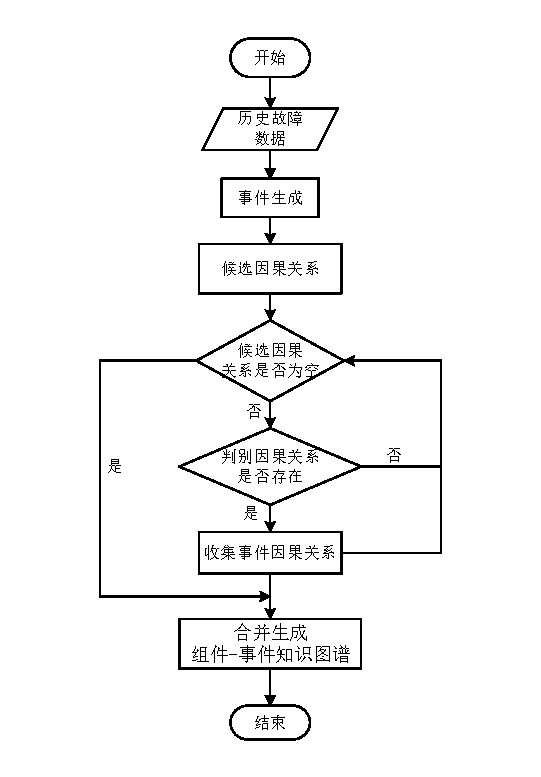
\includegraphics[width=0.65\textwidth]{graph-constructure-process.pdf}
    \caption{组件-事件知识图谱构建程序流程图\label{graph-constructure-process}}
\end{figure}

\subsection{故障预测模块详细实现}
本节介绍故障预测模块的详细实现过程,该过程对应的程序流程如图\ref{failure-predict-process}所示。

在启动故障预测模块后,其会默认一直运行,不停地监测实时事件序列,并给出故障预测结果。当运维人员不需故障预测时,将该功能手动关闭即可。

每当状态监测模块监测到新事件后,最新的1024个事件被输入章节\ref{chapter-predict-failure}所提出的故障预测模型。此时,双向长短期记忆神经网络将实时的事件序列编码成了向量。

随后,本程序遍历知识库中每种故障类型对应的组件-事件知识图谱,与输入的事件序列计算匹配度。当匹配度均小于阈值0.4时,程序会输出集群状态健康的提示;当存在匹配度大于等于0.4的,程序会输出前三的故障预测结果,预测结果为每个匹配的知识图谱对应的故障类型以及其匹配度。本处的阈值0.4是运维人员根据实际运维经验调整设定的。另外,遍历知识库每张知识图谱计算匹配度的过程,同样使用了多线程来加快故障预测速度。
\begin{figure}[htbp]
    \centering
    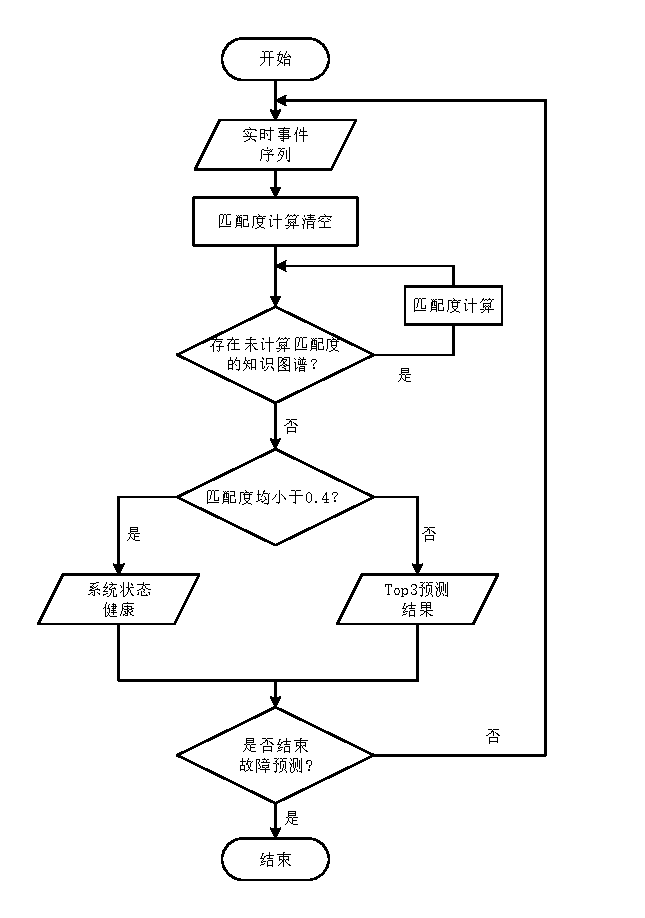
\includegraphics[width=0.65\textwidth]{failure-predict-process.pdf}
    \caption{故障预测程序流程图\label{failure-predict-process}}
\end{figure}

\section{系统测试}
本章根据章节\ref{need-analysis}中所述的功能性需求和非功能性需求,采用JUnit测试框架对系统进行了测试。本节分为5个小节,分别为系统测试环境、运行状态查询测试、组件事件知识图谱查询及调优测试、实时故障预测测试和系统性能测试。
\subsection{系统测试环境}
本章在进行测试前,记录测试过程所在的环境,包括集群、服务器和各种开发工具版本号,如表\ref{system-test-env}所示。
\newpage
\begin{table}[htbp]
    \centering
    \caption{系统测试环境}
    \label{system-test-env}
    \begin{tabular}{cc}
    \toprule[2pt]
    环境项                        & 环境参数                                                                                                                                        \\ \midrule[2pt]
    集群                         & \begin{tabular}[c]{@{}c@{}}集群类型:Kubernetes 托管版\\ 版本:1.12.6-aliyun.1\\ 云服务器个数:30\\ 节点操作系统:CentOS 7.6 64位\\ 节点CPU:8 核\\ 节点内存:16 GiB\end{tabular} \\ \midrule[1pt]
    服务器                        & \begin{tabular}[c]{@{}c@{}}操作系统:Windows 10\\ 处理器:11th Gen Intel(R) Core(TM) i5-11300H\\ 内存:256GB\\ 显存:11GB\\ 硬盘:2TB\end{tabular}            \\ \midrule[1pt]
    Neo4j                      & 版本号4.2.6                                                                                                                                    \\
    Java                       & 版本号1.8.0\_281                                                                                                                               \\
    Python                     & 版本号3.6.8                                                                                                                                    \\
    Kafka                      & 版本号2.2.1                                                                                                                                    \\
    prometheus                 & 版本号2.17.2    \\
    Vue.js                     & 版本号4.5.12    \\
    Spring Boot                & 版本号2.5.0    \\
    \multicolumn{1}{c}{Jaeger} & 版本号1.22.0                                                                                                                                   \\ \bottomrule[2pt]
    \end{tabular}
\end{table}

\subsection{运行状态查询测试}
在进行运维工作时,运维人员会有不同的查询需求,本系统实现了常用的查询方式。本小节对实现的各个运行状态查询功能进行了测试,共设计了4条测试用例,分别对应4种查询功能需求,测试结果如表\ref{test-search}所示。测试结果表明各个查询功能均已正确实现,下面展示各个测试用例在前端界面的返回结果。
\begin{table}[htbp]
    \centering
    \caption{运行状态查询测试用例}
    \label{test-search}
    \begin{tabular}{cc}
    \toprule[2pt]
    内容项  & 描述                                                                                                                                                                                                   \\ \midrule[2pt]
    测试目的 & 测试运行状态查询功能                                                                                                                                                                                           \\ \midrule[1pt]
    前置条件 & 测试机联网、系统查询界面可访问                                                                                                                                                                                      \\ \midrule[1pt]
    用例设计 & \multicolumn{1}{l}{\begin{tabular}[c]{@{}l@{}}1.输入查询语句“vpc slb   ecs”,查询符合特定路径类型的所有拓扑,\\点击查询按钮。\\ 2.输入查询语句“vpc id k1aexj”,模糊查询id 包含k1aexj 的vpc 节点,\\点击查询按钮。\\ 3.鼠标悬停在任一组件上方。\\ 4.鼠标左键点击任一组件。\end{tabular}} \\ \midrule[1pt]
    预期结果 & \multicolumn{1}{l}{\begin{tabular}[c]{@{}l@{}}1.返回查询结果,查询结果为符合“vpc slb   ecs”路径类型的所有拓扑。\\ 2.返回查询结果,查询结果是id包含“k1aexj”子序列的vpc节点。\\ 3.组件右上方浮现该组件的属性信息列表。\\ 4.查询页面右侧弹出该组件的所有指标时序数据。\end{tabular}}        \\ \midrule[1pt]
    测试结果 & 4个用例经过测试与预期结果相符合                                                                                                                                                                                     \\ \midrule[1pt]
    状态   & 通过                                                                                                                                                                                                   \\ \bottomrule[2pt]
    \end{tabular}
\end{table}

图\ref{search-component-path}显示了搜索符合指定路径类型关系的所有拓扑路径。如图所示,在搜索框输入“vpc-slb-ecs”,回车后,下方界面会显示所有符合该路径类型关系的拓扑路径。
% ,height=0.4\textheight
% \begin{figure}[hbtp]
%     \centering
%     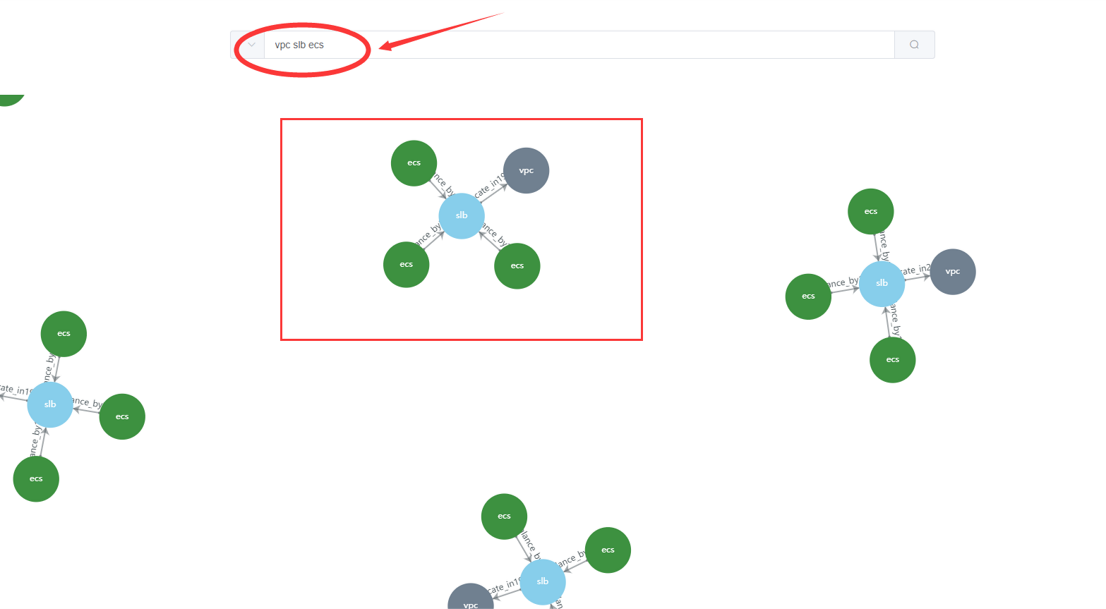
\includegraphics[width=0.75\textwidth,height=0.2425\textheight]{search-component-path.png}
%     \caption{搜索指定路径结果\label{search-component-path}}
% \end{figure}
\begin{figure}[hbtp]
    \centering
    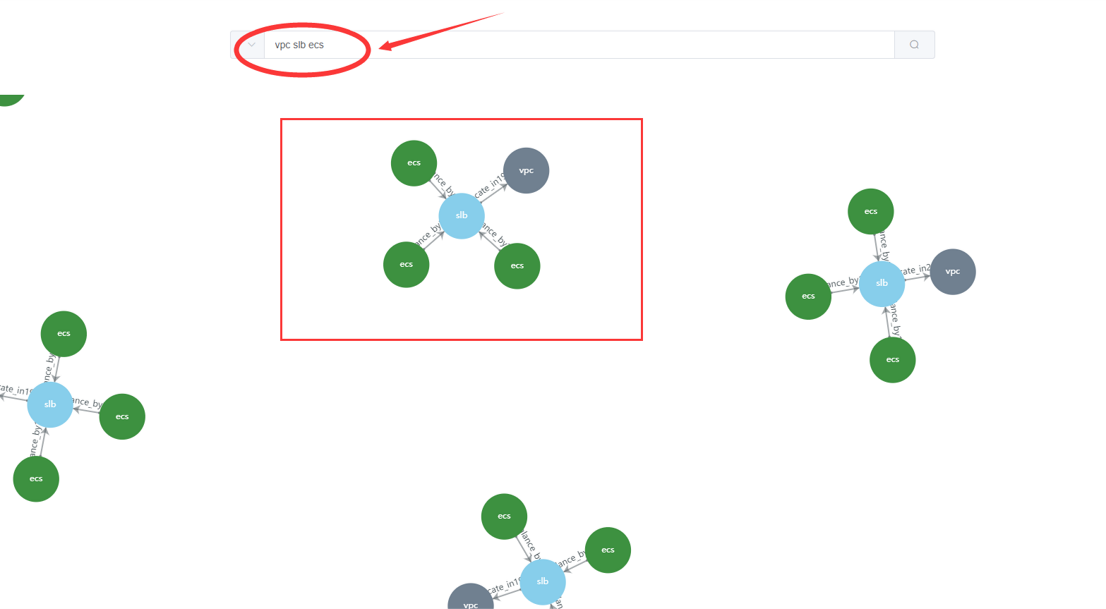
\includegraphics[width=0.8\textwidth,height=0.2425\textheight]{search-component-path.png}
    \caption{搜索指定路径结果\label{search-component-path}}
\end{figure}

图\ref{search-detail-component}显示了模糊搜索符合某类型某id的组件(如id中包含字段k1aexj的VPC组件)。返回结果除了包含符合条件的组件,还包含该组件的周边组件,便于运维人员查看其上下游拓扑。
\begin{figure}[htbp]
    \centering
    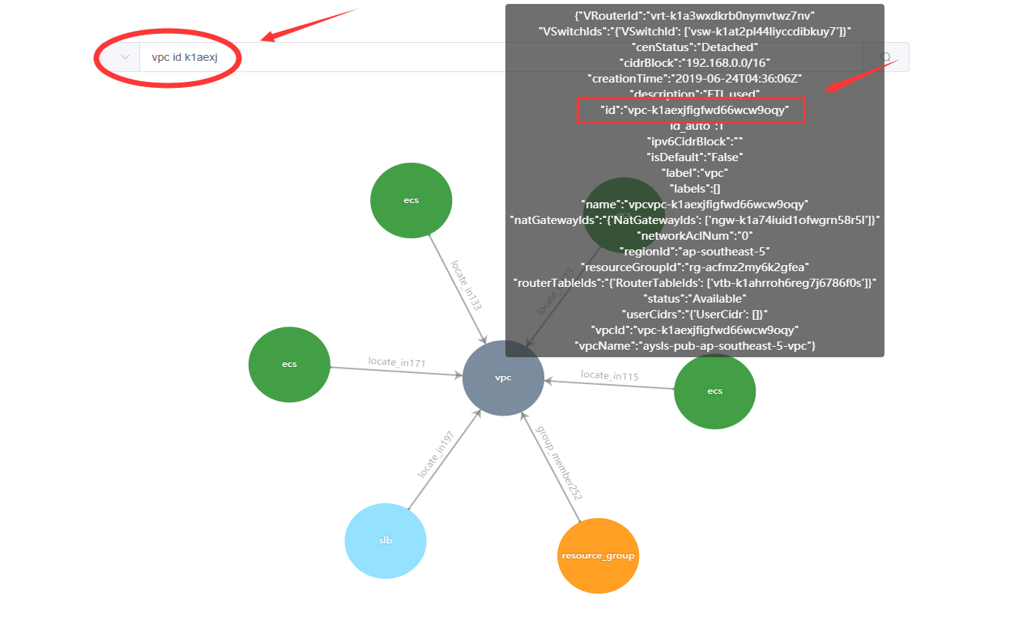
\includegraphics[width=0.9\textwidth]{search-detail-component.png}
    \caption{模糊搜索结点结果\label{search-detail-component}}
\end{figure}

图\ref{component-detail-info}为组件信息显示界面,在该界面中,组件类型、唯一标识和其间拓扑关系都会被直接展示出来。为了显示组件的所有具体属性信息,将鼠标悬停于组件上,右上方的灰色方框中会浮现该组件的属性信息列表。
\begin{figure}[htbp]
    \centering
    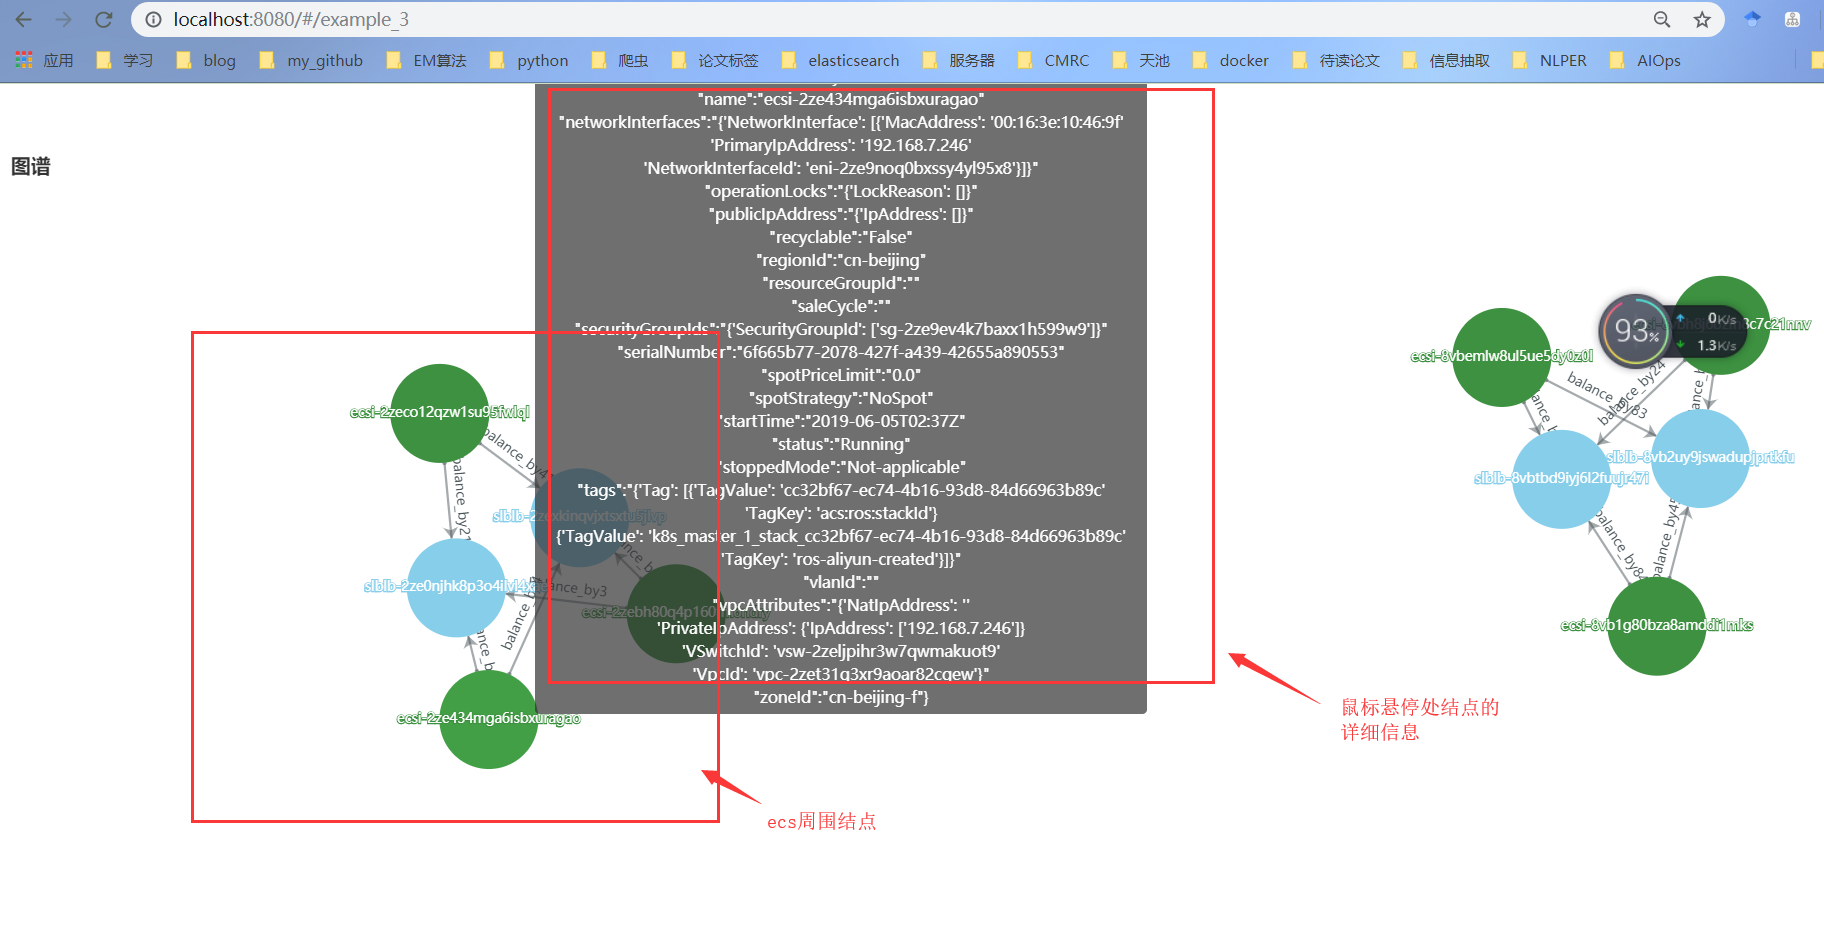
\includegraphics[width=0.9\textwidth]{component-detail-info.png}
    \caption{查询组件属性信息结果\label{component-detail-info}}
\end{figure}

对于组件的指标时序数据,可以通过鼠标左键点击组件,右侧抽屉会弹出该组件的各种指标时序数据折线图。如图\ref{search-component-metric-info}所示,在指标时序数据折线图中,上方会显示该组件的唯一标识,中间有该组件多种指标时序数据类型可以选择,下方横坐标可以任意选择展示区间。
\begin{figure}[htbp]
    \centering
    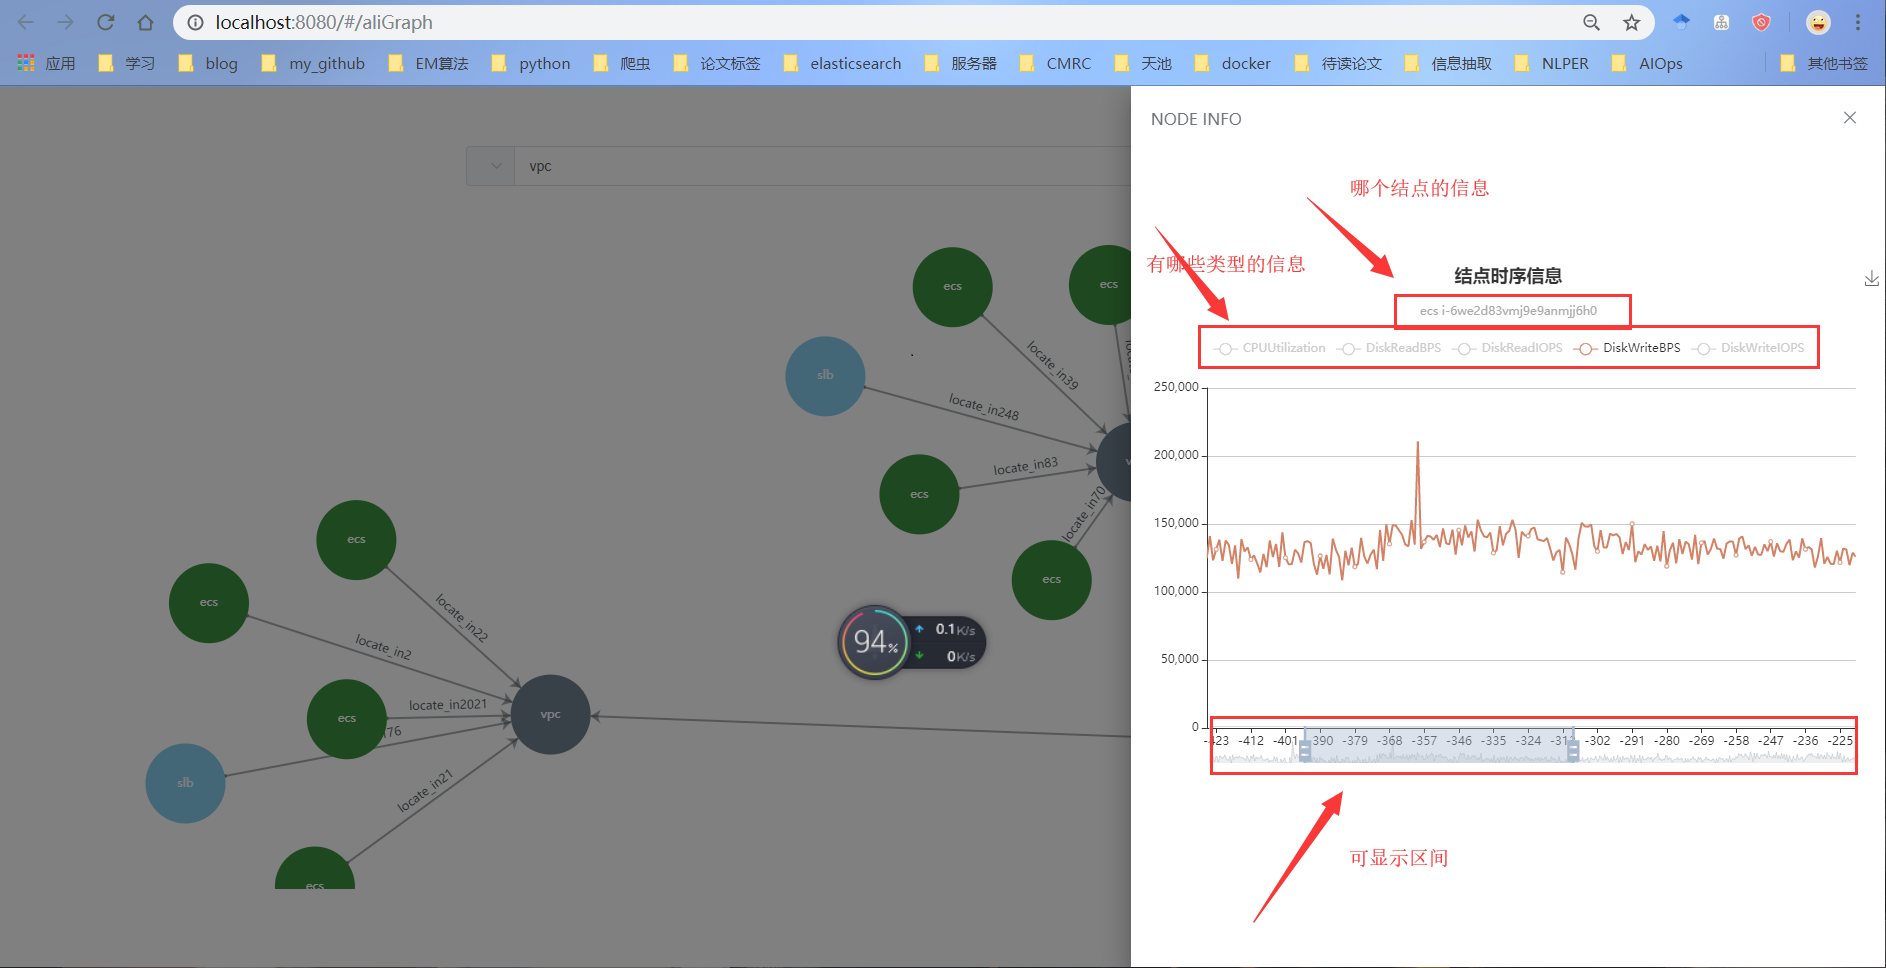
\includegraphics[width=0.8\textwidth]{search-component-metric-info.png}
    \caption{查询组件指标时序信息结果\label{search-component-metric-info}}
\end{figure}

\subsection{组件事件知识图谱查询及调优测试}
本小节对组件-事件知识图谱查询及调优功能进行了测试,共设计了3条测试用例,分别对应查询及调优,测试结果如表\ref{test-graph}所示。
\begin{table}[htbp]
    \centering
    \caption{组件-事件知识图谱查询及调优测试用例}
    \label{test-graph}
    \begin{tabular}{cc}
    \toprule[2pt]
    内容项  & 描述                                                                                                                                               \\ \midrule[2pt]
    测试目的 & 测试组件-事件知识图谱查询及调优功能                                                                                                                               \\ \midrule[1pt]
    前置条件 & 系统已经存在故障代号为f3的组件-事件知识图谱                                                                                                                              \\ \midrule[1pt]
    用例设计 & \multicolumn{1}{l}{\begin{tabular}[c]{@{}l@{}}1.输入查询语句“f3”,查询故障类型代号为f3的组件-事件\\知识图谱,点击查询按钮。\\ 2.左键任一条边,选择删除,并再次查询“f3”。\\3.选择两个事件结点,单击右键添加一条因果关系,并再次查询“f3”。\end{tabular}}             \\ \midrule[1pt]
    预期结果 & \multicolumn{1}{l}{\begin{tabular}[c]{@{}l@{}}1.返回查询结果,查询结果为故障类型代号为f3的组件-事件知识图谱。\\ 2.返回查询结果,删除的边已经不存在于图中。\\3.返回查询结果,添加因果关系存在于图中。\end{tabular}} \\ \midrule[1pt]
    测试结果 & 3个用例经过测试与预期结果相符合                                                                                                                                 \\ \midrule[1pt]
    状态   & 通过                                                                                                                                               \\ \bottomrule[2pt]
    \end{tabular}
\end{table}

图\ref{device-service-event}为查询到的故障代号为f3的组件-事件知识图谱。为了便于查看,整个组件-事件知识图谱使用三层展示:最上层为事件层;中间层为微服务层;下层为部分集群组件层。

\begin{figure}[htbp]
    \centering
    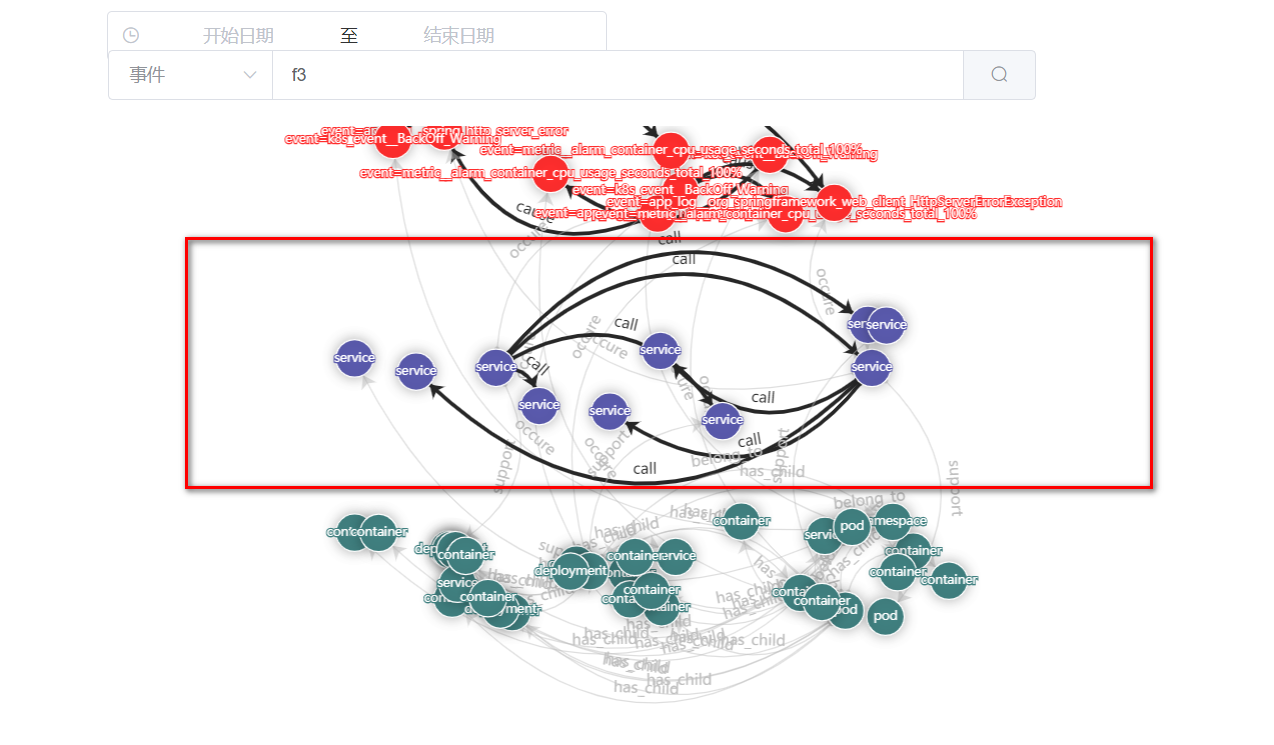
\includegraphics[width=0.8\textwidth]{device-service-event.png}
    \caption{查看f3故障类型的组件-事件知识图谱\label{device-service-event}}
\end{figure}


\subsection{故障预测测试}
本小节对故障预测功能进行了测试,共设计了3条测试用例,测试结果如表\ref{test-predict-failure}所示。
\begin{table}[htbp]
    \centering
    \caption{故障预测测试用例}
    \label{test-predict-failure}
    \begin{tabular}{cc}
    \toprule[2pt]
    内容项  & 描述                                                                                                                                           \\ \midrule[2pt]
    测试目的 & 故障预测功能                                                                                                                                       \\ \midrule[1pt]
    前置条件 & 系统存在组件-事件知识图谱,开启了故障检测功能                                                                                                                      \\ \midrule[1pt]
    用例设计 & \multicolumn{1}{l}{\begin{tabular}[c]{@{}l@{}}1.开启故障预测功能,后台注入f3故障的根因异常。\\ 2.关闭故障预测功能,后台注入f3故障的根因异常。\\ 3.开启故障预测功能,后台不注入任何异常。\end{tabular}}   \\ \midrule[1pt]
    预期结果 & \multicolumn{1}{l}{\begin{tabular}[c]{@{}l@{}}1.在故障产生前,页面弹出故障预测top3结果及其对应匹配\\ 度值。\\ 2.故障预测页面未出现任何信息。\\ 3.故障预测页面,一直显示“集群状态健康”。\end{tabular}} \\ \midrule[1pt]
    测试结果 & 3个用例经过测试与预期结果相符合                                                                                                                             \\ \midrule[1pt]
    状态   & 通过                                                                                                                                           \\ \bottomrule[2pt]
    \end{tabular}
\end{table}

图\ref{failure-prediction}为实时故障预测界面。在该界面中,实时数据同样以三层结构展示,但发生异常事件的微服务、系统组件节点会显示为红色。当实时数据经过后台故障预测模型判别会出现故障时,右边会弹出故障预测结果窗口,并按照故障类型匹配度由高至低排出前3个最匹配的结果。事件层会显示可能的故障触发链条。
\begin{figure}[htbp]
    \centering
    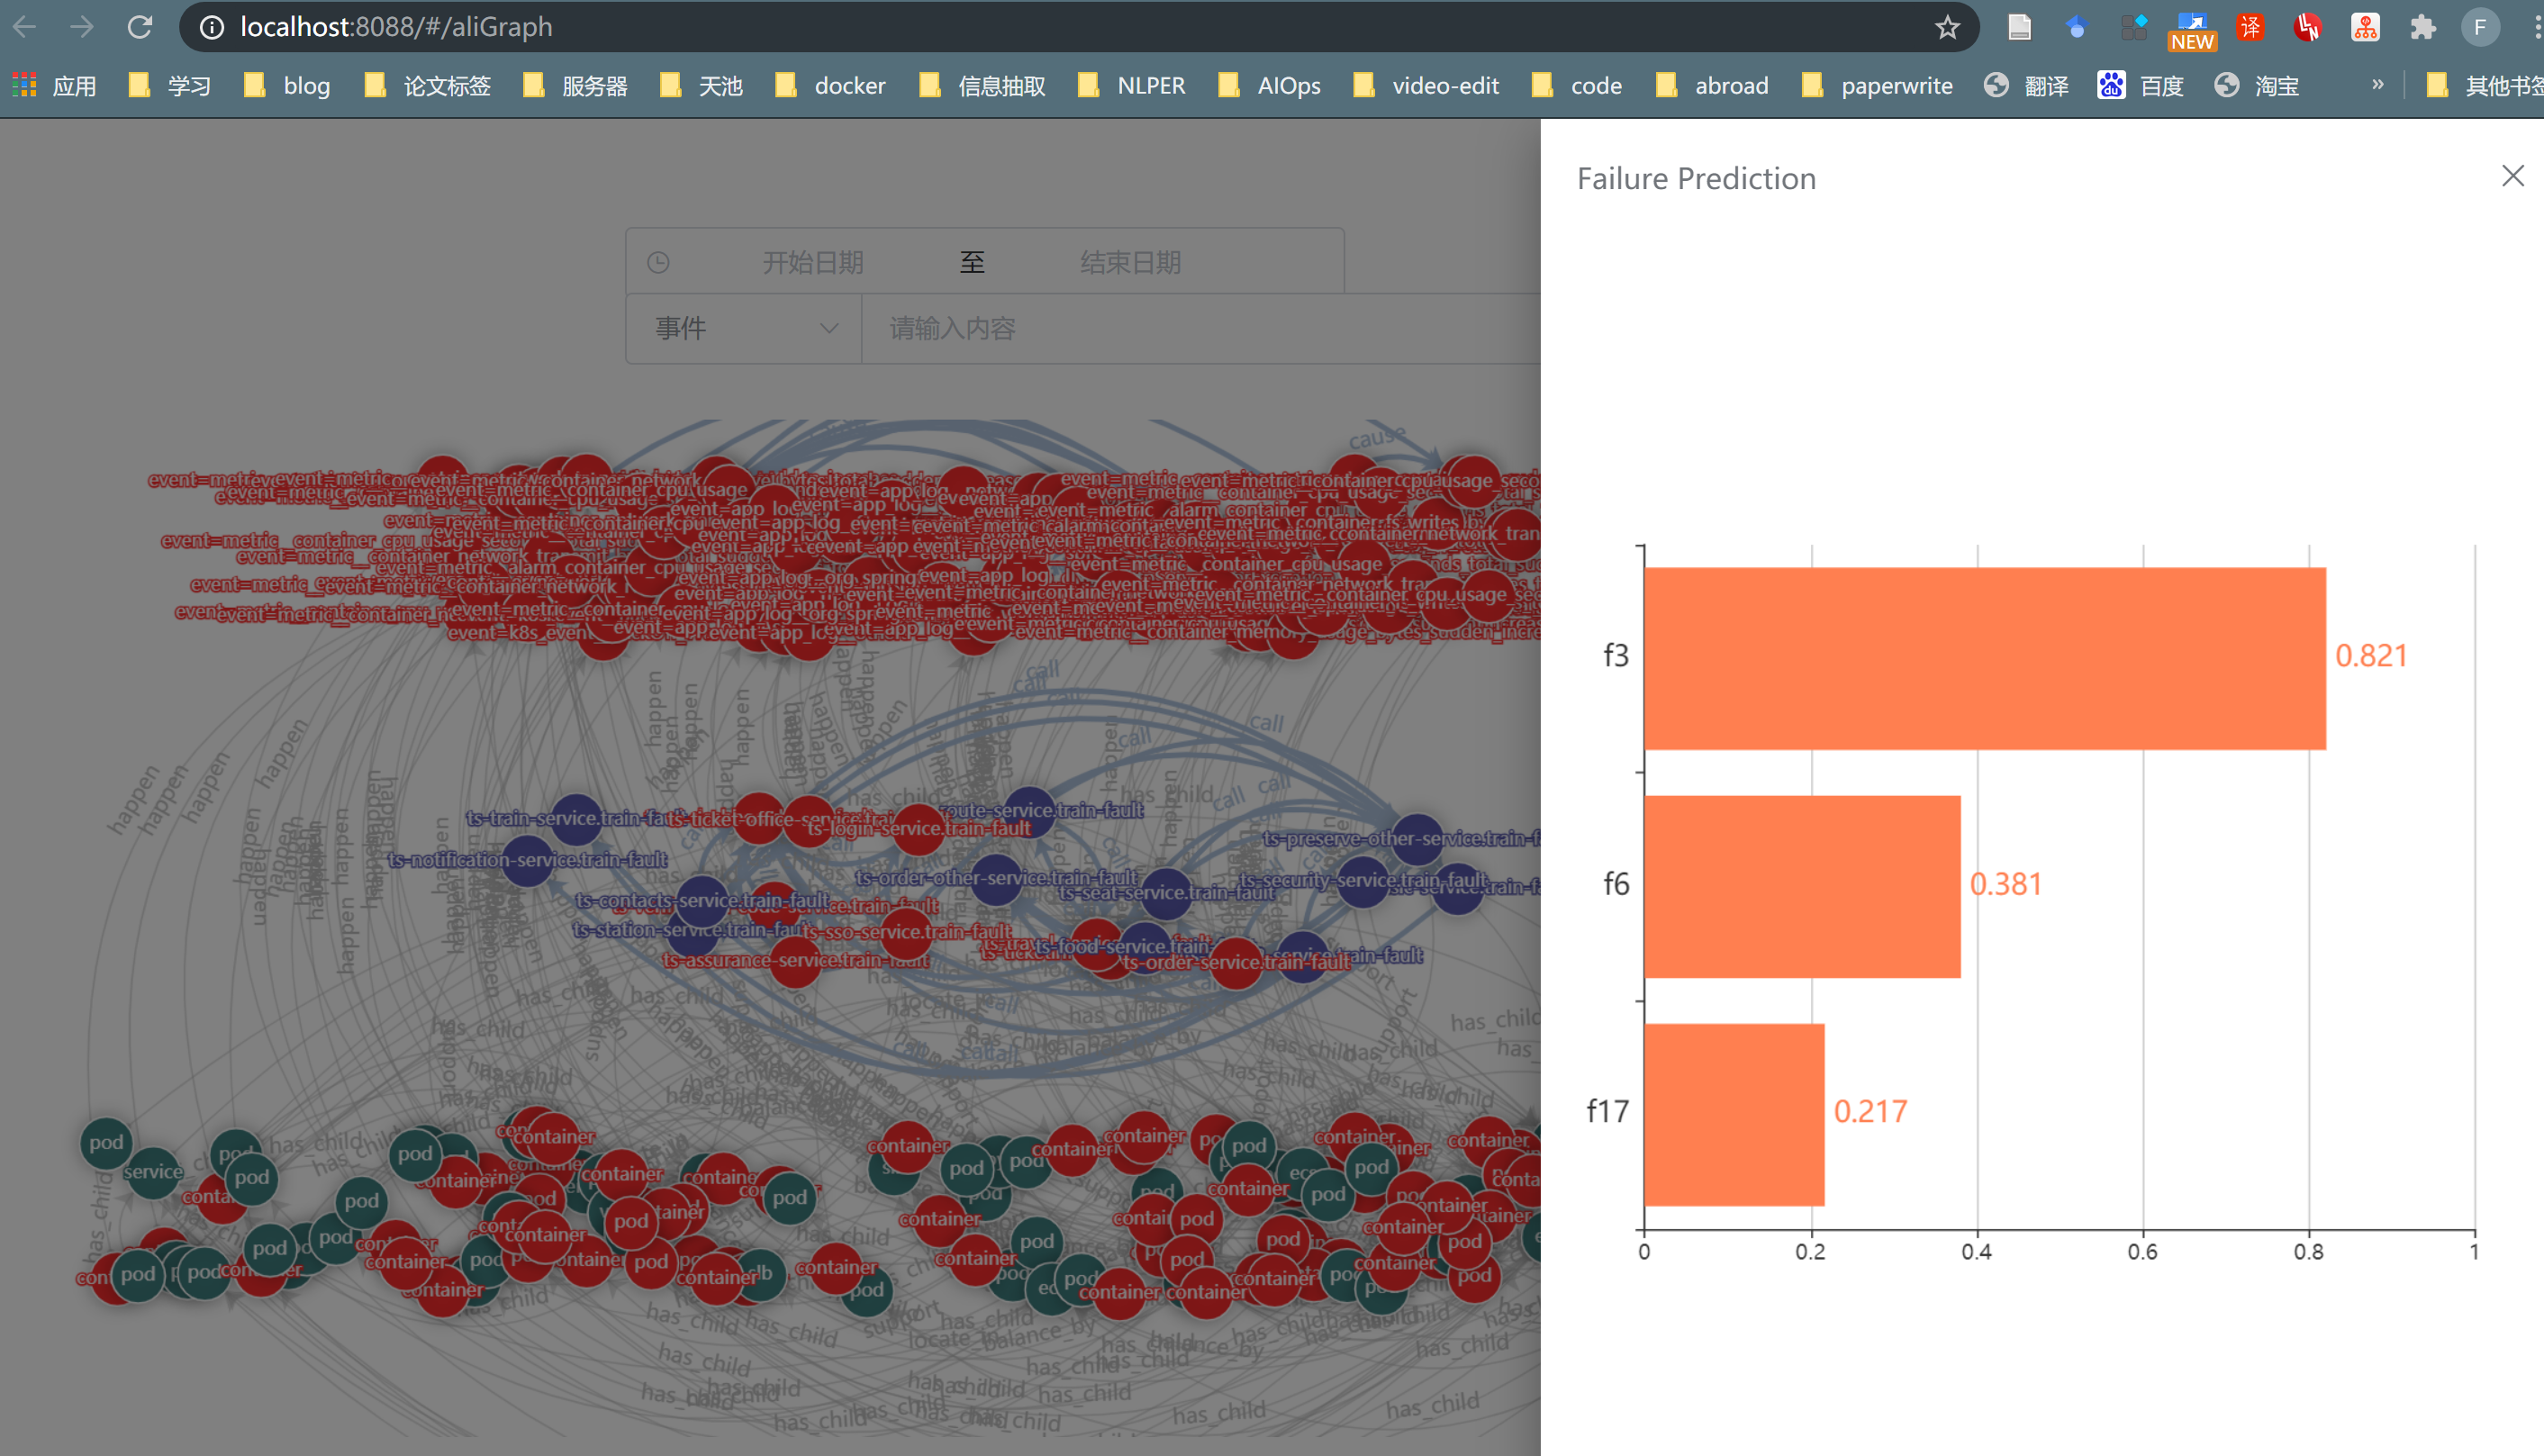
\includegraphics[width=0.8\textwidth]{failure-prediction.png}
    \caption{实时故障预测结果\label{failure-prediction}}
\end{figure}

\subsection{系统性能测试}
本节测试了系统的性能表现,主要包括各个查询功能和故障预测的时间消耗。本节对每一个测试项重复了100次,最终以平均耗时作为测试结果,如表\ref{test-performance}所示。由测试统计结果可见,本系统满足了秒级的系统性能需求。
\begin{table}[htbp]
    \centering
    \caption{系统性能测试}
    \label{test-performance}
    \begin{tabular}{cc}
    \toprule[2pt]
    系统性能测试项                                                      & 时间消耗  \\ \midrule[2pt]
    查询特定路径类型的拓扑                                                  & 1.71s \\\midrule[1pt]
    模糊查询某个组件                                                     & 1.59s \\\midrule[1pt]
    悬停显示组件信息                                                     & 0.76s \\\midrule[1pt]
    \begin{tabular}[c]{@{}c@{}}左键获取组件\\ 指标时序数据\end{tabular}      & 1.65s \\\midrule[1pt]
    \begin{tabular}[c]{@{}c@{}}搜索某故障类型的\\ 组件-事件知识图谱\end{tabular} & 0.63s \\\midrule[1pt]
    \begin{tabular}[c]{@{}c@{}}注入异常到故障预测\\ 正确并弹出结果\end{tabular}  & 2.38s \\ \bottomrule[2pt]
    \end{tabular}
\end{table}

\section{本章小结}
本章分析了IT运维人员在实际工作中的需求,根据第三章、第四章和第五章所提出的各个算法模型,设计了一个基于知识图谱的IT运维辅助系统。随后,本章详细实现了多个功能模块,使得系统可以快速整合多源异构数据、自动沉淀生成组件-事件知识图谱,进行实时故障预测。最后,经过系统测试,证明了本系统可以满足IT运维人员的实际工作需求。
